\chapter{Shape Sensitivity Analysis using Immersed Boundary Method}
In this chapter we apply the continuum sensitivity analysis to the CFD simulations conducted using the Immersed Boundary (IB) method. In this chapter the focus is on calculating the sensitivity of flow variables such as pressure and velocity to the design variable that controls the shape of the boundary, i.e. radius of a cylinder, camber of an airfoil. The boundary of the solid domain is represented using an analytical function. However, as will be shown in the following chapters this is not a required for this method. In this chapter the modifications on the IB approach to make it suitable for continuum sensitivity formulation is discussed. To the best of the author's knowledge, this is the first time that sensitivity analysis is done for CFD simulations based the continuum IB formulation.
% ======================================================================================
\section{Sensitivity Problem Formulation}
In contrast to traditional body conformal methods, in IB approach the solid boundaries are represented by modifying the governing equation near the boundaries. In the case of continuum IB method, this is done by adding the appropriate force term to the cells adjacent to the immersed boundary. The value of these forces are calculated either using a feedback forcing \cite{goldstein1993modeling} or a penalization function \cite{arquis1984conditions}. The Navier-Stokes (NS) equations are written as shown in Equation \eqref{eq:C4_NS}.

\begin{equation}\label{eq:C4_NS}
	\frac{\partial \mathbf{u}}{\partial t} + \mathbf{u} \cdot \nabla \mathbf{u} = 
	-\frac{\nabla P}{\rho} + \mu \nabla^2 \mathbf{u} + \mathbf{f}
\end{equation}

where $\mathbf{u}$ is the velocity vector, $P$ is pressure, $\mu$ is the kinematic viscosity ($\mu / \rho$), $\rho$ is density, and $\mathbf{f}$ is the forcing term. The NS equations are solved on a Eulerian grid that is fixed in space and the IB is defined on a separate Lagrangian grid that can move. This is shown Figure \ref{fig:C4_lagrangianAndEulerianDomain}.

\begin{figure}[h]
	\centering
	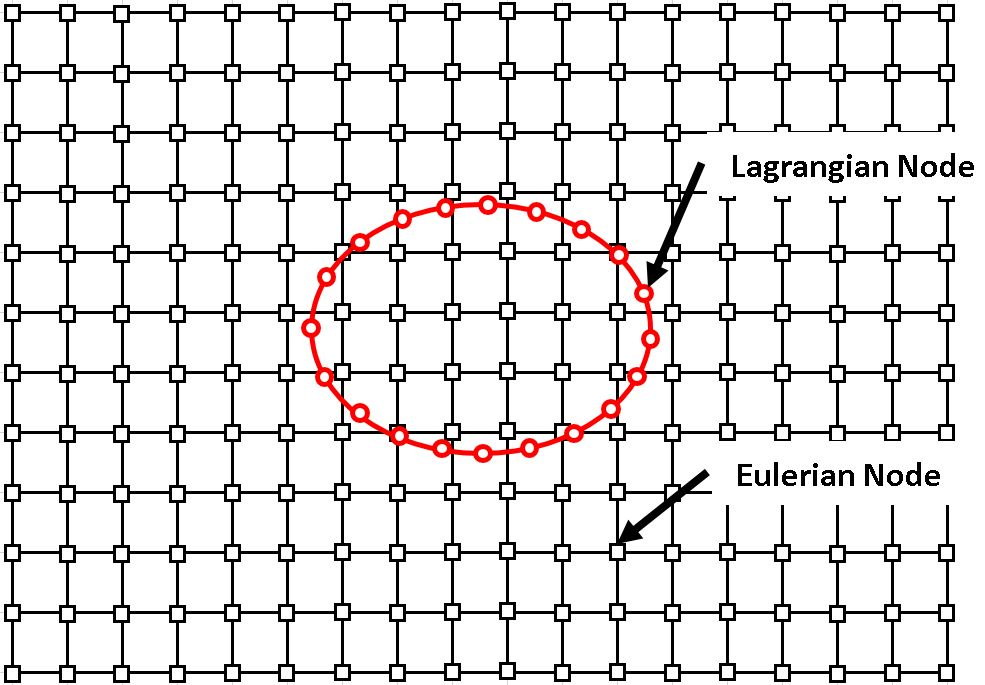
\includegraphics[width=7.00cm]{Chapter_4/figure/lagrangian_and_eulerian_nodes.jpg}
	\caption{Eulerian and Lagrangian nodes for representing the fluid and solid domain. The Eulerian and Lagrangian nodes are represented by black squares and red circles.}
	\label{fig:C4_lagrangianAndEulerianDomain}
\end{figure}

The forcing function in the penalization method is calculated at the Eulerian nodes and is applied to computational nodes inside the solid boundary using a step function as shown in Equation \eqref{eq:C4_penalizationForcingFunction}.

\begin{equation}\label{eq:C4_penalizationForcingFunction}
	\mathbf{f} = -\mathcal{S}(\mathcal{X}) \kappa \mathbf{u}
\end{equation}

where $\mathcal{S}$ is the step function, $\mathcal{X}$ defines the relative location of locations inside the domain with respect to the IB boundary, $\kappa$ is the penalization parameter, and $\mathbf{u}$ is the fluid velocity.

\begin{equation}\label{eq:C3_feedbackForcingFunction}
	\mathbf{f}(\mathbf{X}, t) = 
	\alpha \int_0^t \left[ \mathbf{u}(\mathbf{X}, \tau) - \mathbf{V}(\mathbf{X}, \tau) \right] d\tau + 
	\beta \left[ \mathbf{u}(\mathbf{X}, \tau) - \mathbf{V}(\mathbf{X}, \tau) \right]
\end{equation}

\subsection{Regularized Delta/Heaviside Function}

\subsection{Direct Method}

\subsection{Adjoint Method}

\section{Shape Sensitivity Analysis for 1D problem}

\section{Shape Sensitivity of Flow over a Cylinder}

\section{Shape Sensitivity of Flow through a Nozzle}

\section{Summary}
